\chapter{Methodology}
In this chapter, we discuss the proposed method to address the issues which have been observed in previous chapter. As we have seen there are lot of active queue management schemes intend to control the congestion in the network but that does not exploit the spatial correlation between the nodes. To resolve it, an algorithm has been proposed which will be discussed in this chapter. We will validate the algorithm by analytical approach through queuing models. The algorithm has been explained with the help of a flowchart. Finally the chapter ends with concluding remarks. 
\section{Proposed hypothesis}
Our approach can be explained by the flowchart in the Figure 3.1 and the notations used in the flowchart are described in Table 3.1.
\begin{enumerate}
    \item At any node, arrival of a packet marks the beginning of algorithm. Before beginning the algorithm, we need to define two thresholds, minimum threshold min\textsuperscript{th} and max\textsuperscript{th}, for minimum and maximum threshold respectively. 
    \item When any packet, let's say \textit{n}, arrives at any node, it checks for whether the queue at the node is empty, partially filled or completely filled. If the buffer is empty or the buffer size is less than the min\textsuperscript{th}, the packet is enqueued in the buffer.
    \item However, when the buffer size is between the min\textsuperscript{th} and max\textsuperscript{th}, the packet is checked for the spatial correlation between the incoming packet and the packets already queued in the buffer. 
    \item The factors checking for the spatially correlated redundant packets are time elapsed between the arrival of two packets, and the euclidean distance between the source nodes along with the data in the packets.
    \item If the time elapsed between the arrival of two packets is less than the defined threshold, drop probability is assigned to the packet on the average queue length. The average queue length is calculated as a function of the queue weight at any instant. However, if the time elapsed between the two packets is equal or greater than the defined threshold, the factors for spatially correlation between the packets are checked for. 
    \item Finding the spatial correlation between the packets, the packet is dropped, else the drop probability for packet is assigned on the basis of the value of information, i.e. the correlation between the packets is used as a drop probabilty for the packet. 
\end{enumerate}
\begin{table}[h!]
\begin{center}
\caption{Notations used in the flowchart}
\begin{tabular}{p{2.0cm} p{10.0cm} }
\hline
buff\_size & Size  of  the  Buffer\\ 
min\_th &  Minimum  Threshold  for  the  buffer  queue \\
max\_th & Minimum  Threshold  for  the  buffer  queue.  Generally  equal  to  the  buff\_size \\
time\_elapsed & Time  interval  between  the  arrival  of  two  consecutive  data  packets \\
defined\_th &  Average  permissible  delay.  Taken  as  one  hop  delay \\ payload\_diff &  difference  between  the  payload  of  two  consecutive  packets \\
PD & drop  probability  assigned  to  each  packet \\
\hline
\end{tabular}
\end{center}
\end{table}
The flowchart distinguishes between the proposed hypothesis and the conventional approach. The drop probability in traditional approach is based on the FCFS policy, i.e. the packets arriving are assigned probability on the basis of their arrival.\
\begin{figure}
    \centering
    \includegraphics[height=16cm, width=11cm]{Thesis/figs/FLOW.png}
    \caption{Work Flow}
    \label{fig:my_label}
\end{figure}

\section{Mechanism/Algorithm}
The main objective of the algorithm is to find the redundant packets and assign them higher probability. 
\begin{algorithm}[h!]
\caption{Proposed scheme}
\begin{algorithmic}[1]
\Procedure{}{}
\State $avg \gets \textit{average queue length}$
\State $count \gets \textit{number of packets arriving since last packet marked }$
\BState \emph{for each packet arrival}:
\State \textit{calculate the new avg. queue size}
\If {$buffer \neq \textit{empty}$} 
\State $avg \gets (1-w\textsubscript{q}) \times avg + w\textsubscript{q} \times q $  
\Else 
\State $m \gets f(time-q\_time)$
\State $avg \gets (1-w\textsubscript{q}) \times m \times avg $
\EndIf
\If {$minth \leq avg \leq maxth$}
\State increment count
\State calculate c\textsubscript{r}
\State calculate probability p\textsubscript{a}:
\State $p\textsubscript{b} \gets maxp \frac{avg-minth}{maxth-minth}$
\State $p\textsubscript{a} \gets \frac{p\textsubscript{b}}{1-count \times p\textsubscript{b}}$
    \If{$c\textsubscript{r} \geq 0.5$}
    \State $P\textsubscript{d} \gets c\textsubscript{r}$
    \Else
    \State $P\textsubscript{d} \gets p\textsubscript{a}$
    \EndIf
\Else{ $avg \geq maxth$}
    \State mark the arriving packet with probability p\textsubscript{a}
    \State $count \gets 0$
\EndIf
\EndProcedure
\end{algorithmic}
\end{algorithm}
The algorithm computes the average queue size at packet arrivals, rather than at fixed time intervals, the calculation of the average queue size is modified when a packet arrives at the router to an empty queue. After the packet arrives to an empty queue the algorithm calculates m, the number of packets that might have been transmitted by during the time that channel line was free. It calculates
the average queue size as if m packets had arrived with a queue size of zero.\\
Two parameters, minth (minimum threshold) and maxth (maximum threshold) are used to decide the marking probability,minth specifies the average queue size below which no packets will be marked, while maxth specifies the average queue size above which all packets will be marked. As the average queue size varies from minth to maxth, packets will be dropped with a probability that depends on the correlation an arriving packet has with the previously enqueued packed i.e.c\textsubscript{r}.
\subsection{Analysis of Algorithm}
While analyzing an algorithm, we mostly consider time complexity and space complexity. Time complexity of an algorithm quantifies the amount of time taken by an algorithm to run as a function of the length of the input. The time complexity of the proposed algorithm can be calculated as:
\begin{equation}
Running time(algo)= Running time(For loop) \times Running time(Body)   
\end{equation}
\begin{itemize}
    \item Running time(For loop)
    \newline For loop in line (4) will run for n packets that arrive into the queue. Therefore 
    \begin{equation}
     RunningTime(For loop)=O(n)  
    \end{equation}
    \item Running time(Body): Since all the if-else blocks contain operation that would take constant time, irrespective of number of inputs. The time taken is constant. 
\end{itemize}       
Therefore from Equation 3.1 and 3.2, the running time of algorithm can be given as:
\begin{equation}
    Time\_Complexity(Algorithm) = O(n) \times c = O(n)
\end{equation}
The correctness for any algorithm can be proved by considering all the possible input and their corresponding outputs. For each input, the algorithm must be able to produce definite results in a finite time. For the proposed algorithm, the input can be taken as any arriving packet and the desirable output is a definite drop probability provided to it. 
\begin{itemize}
    \item {\bf Input:} Arriving packet.
    \item {\bf Output:} Packet given a drop probability.
\end{itemize}
    \begin{itemize}
        \item {\bf Case 1: When the queue is empty}
            \newline If the arriving packet sees the buffer is empty,its average queue is calculated as a function of the the number of packets that could have been transmitted during the time. The packet is marked with zero probability.
        \item {\bf Case 2: When the queue length is between maximum and minimum threshold}
        \newline
         When the data is highly correlated, packet is marked with the probability equal to the correlation coefficient. 
         \newline When the data is not correlated,it is marked with the probability as a function of the average queue length.
       \item {\bf Case 3: When the queue length exceeds the maximum threshold} 
    \newline The packet is marked with the probability which is a function of the average queue length. 
\end{itemize}
In all the above possible three cases, the packet is being marked with a probability. 
\section{Analytical validation}
This section presents the queuing model for the proposed hypothesis and a comparative analysis is done between the proposed hypothesis and the traditional approach. Summary of symbols used in the validation proof is given in Table 3.2.
\begin{table}[h]
\begin{center}
\caption{Summary of important symbols}
\begin{tabular}{p{1.0cm} p{10.0cm} }
\hline
 $\lambda$ & packet arrival rate at any node i \\ 
 $\mu$ & packet service rate at any  node i\\
 P \textsubscript{0} & Probability of zero packets in the queue at any instant\\
  P \textsubscript{n} & Probability of n number of packets in the queue at any instant\\
 $\rho$ & Utilization factor of the system\\
 k & maximum buffer capacity at any node\\
\hline
\end{tabular}
\end{center}
\end{table}
\subsection{Queuing model}
Consider a wireless sensor network consisting of N nodes. The network is synchronized and fault tolerant. The nodes have sufficient memory to share any amount of data. The packets are independent and only dropped in the network due to buffer overflow. Let the time interval upon consideration be t and t +$\Delta$t. During this time, there can be multiple arrivals at the intermediate node from different source as shown in the Figure 3.2. 
\begin{figure}[H]
    \centering
    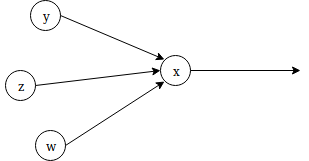
\includegraphics[height=5cm]{Thesis/figs/1.png}
    \caption{Multiple path routing }
    \label{fig:my_label}
\end{figure}
\par 
The arrival of packets is a random process. Therefore, the arrival pattern of packets can be modelled as a Poisson process. The queueing model is represented as shown in Figure 3.3. The service time can be modelled as exponential distribution i.e. packet length distribution. Hence, the system can be mathematically modelled as M/M/1 queuing model with finite buffer capacity K (Based on Kleinrock’s Independent assumption).
\vspace{0.5cm}
\begin{figure}[H]
    \centering
    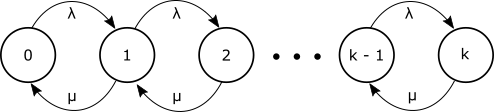
\includegraphics[height=2.5cm, width=15cm]{Thesis/figs/MM1.png}
    \caption{M/M/1 queuing model at a node}
    \label{fig:my_label}
\end{figure}
{\bf Kleinrock's Independent assumption\footnote{Klienrock's Independent assumption has been explained in detail in Appendix B.}} states that {\bf It is often appropriate to use M/M/1 queues for each communication links when the arrivals at entry points are Poisson, the length of the packets are roughly exponential, network is dense and traffic is heavy.} 
\newline
The buffer can be modelled as M/M/1/k queue.The average  number of packet in the system (L \textsubscript{s})
can be calculated as:
\begin{equation}
\begin{split}
L \textsubscript{s} & = E [N] \\
 & = \sum_{n=0}^{k} n (\frac{\lambda}{\mu})^n  P \textsubscript{0}\\
 & = \frac{\rho}{1-\rho}-\frac{(k+1) (\rho)\textsuperscript{k+1}}{1-(\rho)\textsuperscript{k+1}}
 \end{split}
 \end{equation}
Therefore, average number of the packets in queue can be given as:
\begin{equation}
\begin{split}
L \textsubscript{q} & = E [N-1] \\
 & = \sum_{n=1}^{k} (n-1) P \textsubscript{n} \\
 & = \sum_{n=1}^{k} n P \textsubscript{n} - \sum_{n=1}^{k} P \textsubscript{n} \\
 & = E(N)
 - (1- P \textsubscript{0}) \\ 
\end{split}
\end{equation}
\begin{equation}
    L \textsubscript{q} = L \textsubscript{s}-(1- P \textsubscript{0})
    \end{equation}
Probability of a packet drop P\textsubscript{d}:
\begin{equation}
    P\textsubscript{d}= P\textsubscript{k}+ \Gamma
\end{equation}
where 
\newline
P\textsubscript{k} = packet is dropped when the buffer gets full.
\newline
$\Gamma$ = packet is dropped when it is correlated.
\newline
The probability that a packet is dropped when the buffer gets full is given as:
\begin{equation}
    P\textsubscript{k} = \rho^k \Pi \textsubscript{0}
\end{equation}
\begin{equation}
\rho=\frac{\lambda}{\mu}
\end{equation}
Sensing area for a node S, will be given as:
\newline
\centerline{$Area \textsubscript{S} =4\Pi{r}^2$}
Assume two nodes A and B having sensing area A\textsubscript{r} and B\textsubscript{r}, transmitting the data to the third sensor. The meaningful data will be given as:
\newline
\centerline{$\alpha(A\textsubscript{r} \cup B\textsubscript{r})$} 
where $\alpha$ is a proportionality constant; sensing factor of nodes.
\newline
The amount of redundant data will be given as:
\newline
\centerline{$\alpha(A\textsubscript{r} \cap B\textsubscript{r})$} 
{\bf Correlation between sensed data by two nodes A and B can be given as: }
\begin{equation}
\Gamma= \frac{\alpha(A\textsubscript{r} \cup B\textsubscript{r})}{\alpha(A\textsubscript{r} \cap B\textsubscript{r})}
\end{equation}
As the probability of a packet being dropped consists of two factors P\textsubscript{k} and $\Gamma$, {\bf the average number of packets in the queue L\textsubscript{q} decreases.}
\newline
This, in turn, {\bf reduces the waiting time for the packets in queue}:
\begin{equation}
    W\textsubscript{q} = \frac{L\textsubscript{q}}{\widetilde{\lambda}}
\end{equation}
\newline where, 
\begin{equation}
    \widetilde{\lambda} = \mu (1-\Pi \textsubscript{0})
\end{equation}
as the arrival  will be justified as long as the buffer is empty.
\section{Conclusion}
In this chapter, we have discussed the proposed design to handle the redundant transmissions in the network. The whole of the proposed architecture has been clearly explained with the help of a flowchart. The Proposed scheme to handle the spatially correlated data has been discussed in the chapter. Proposed algorithm has been analyzed by studying its time complexity and correctness. An analytical model have been discussed which proves proposed scheme to be better than the existing approach. 
To conclude, we may say that the proposed scheme, mathematically has many advantages over the existing approaches.In the next chapter, we will be validating the proposed model by performing simulations on Network Simulator tool.  Performance of the system will  be measured for various metrics and results will be concluded.